\documentclass[UTF8]{article}
\author {Dis \cdot {count}}

\title {非平衡博弈的一个实例-机器调度博弈}
\date{}

\usepackage{ctex}
\usepackage{amsmath}
\usepackage{amsthm}


\usepackage{geometry}
\geometry{a4paper,scale=0.8}
\usepackage{graphicx}
\usepackage{amssymb}

\usepackage{setspace}
\renewcommand{\baselinestretch}{1.5}


\newtheorem{thm}{\hspace{2em}定理}
\newtheorem{lem}{\hspace{2em}引理}
\newtheorem{pf}{\hspace{2em}证明}
% \newtheorem{def}{\hspace{2em}定义}

\begin{document}
    \maketitle

%  \begin{abstract}
% \end{abstract}

\qquad \textbf{关键词: 合作博弈、成本分摊、机器调度博弈}

\section{基本概念}
我们先来介绍一些准备知识如下。可转移效用的合作博弈模型可以描述为一对参数 $(V,c)$,其中 $V=\{1,2,\dots,v\}$ 表示 $v$ 个参与者的集合,并且 $v\geq2$,同时
$c:2^{V}\to \mathbb{R}$ 表示一个特征函数。一个联盟被定义为一个参与者非空的子集,并且 $V$ 表示大联盟。我们使用 $S=2^{V} \setminus\{\emptyset\}$ 表示所有联盟的集合。对于每个联盟 $s\in S$, 特征函数 $c(s)$ 是当联盟 $s$ 中的成员合作时完成他们工作所需的最小总花费。合作博弈需要一个成本分配向量 $\alpha=[\alpha_{1},\alpha_{2},\dots,\alpha_{v}] \in \mathbb{R}^{v}$ 其中 $\alpha_{k}$ 代表参与者 $k \in V$ 的成本分配。我们使用 $\alpha(s)=\sum_{k\in{s}}\alpha_{k}$ 来简记每个联盟 $s\in S$ 的总成本。
合作博弈中一个最重要的概念是核,记为核 $(V,c)$,即满足平衡预算限制,$\alpha(V)=c(V)$ 和联盟稳定限制 $\alpha(s) \leq c(s)$ 的成本分配向量 $\alpha\in\mathbb{R}^{v}$ 的集合。或者说,我们有 $Core(V,c)= \left\{\alpha:\alpha(V)=c(V), \alpha(s)\leq c(s)\ \text{对所有}\ s \in S \setminus\{V\}, \alpha \in \mathbb{R}^{v} \right\}$。
我们可以采用补贴的方式,即中央集权对选择在大联盟中合作的成员提供一定的补贴,使得在所有成员中分摊的总成本少于 $c(V)$。
所需要的最小补贴可以用下式表示:
\begin{equation} \label{model}
  \omega^*=\mathop{\min}_{\alpha}\{c(V)-\alpha(V):\alpha(s)\leq c(s)\ \text{对所有}\ s \in S, \alpha\in\mathbb{R}^{v}\}
\end{equation}
为了体现出设施定价(征税)对补贴的影响,我们定义特征函数
\[
c(s,m(s,P))=\mathop{\min}\{cx+Pm:Ax \geq By^s+D, \tilde{\alpha}x \leq m,x \in \mathbb{Z} ,m \in \mathbb{Z}\} ,\text{其中} s \in S
\]
其中P表示公共设施的定价,m为公共设施数目。同时,我们称$c(s)$中的 $c_0(s) = cx$ 部分为时间成本,因为这部分是$t_i$的函数,而 $Pm$ 部分为设施成本。
我们的目标是在给定设施定价的情况下,得到在大联盟中的成员需要分担的最小成本,其中通过提高定价(征税)的方式作为补贴以稳定整个大联盟则为我们的主要兴趣所在。而在此之前,我们将研究设施价格会如何影响补贴值。

对于(\ref{model})式,作为一种常用的技巧,拆分$c(s)=c_0(s)+m_sP, s \in S$, 我们将得到它的对偶问题的表示式如下:

\begin{equation} \label{dual}
  \omega(P)=\mathop{\max}_{\rho}\{c_0(V)+m_vP+\sum_{s\in S\setminus\{V\}}-\rho_s[c_0(s)+m_sP]:\sum_{s\in S\setminus\{V\}:k\in s}\rho_s=1,\forall k \in V,\rho_s\geq 0,\forall s \in S \setminus{V}\}
\end{equation}

对于(\ref{dual})式,此时我们可以看出,当$m_v $为某个固定整数时,$\omega(P)$是一组直线的逐点最大值,即意味着$\omega(P) $在对应的区间是凸函数,并且在 $P$ 处的斜率为 $m_v-\sum_{s\in S \setminus\{V\}} \rho_s \cdot m_s$。

同时对于任何联盟 $s\in S\setminus{V}$,都有 $\alpha(s,P)\leq c(s)+m_sP$。特别地,我们称满足 $\alpha(s,P)=c(s)+m_sP$ 的联盟为最不满意联盟。同时定义 $S^{\alpha P}=\{s_1^{\alpha P},s_2^{\alpha P},\dots,s_h(\alpha,P)^{\alpha P}\}$ 表明所有不满意联盟的集合,其中 $h(\alpha,P)=|S^{\alpha P}|$。
由此我们可以得到下式:$s_1^{\alpha P}\cup s_2^{\alpha P}\cup\dots\cup s_h(\alpha,P)^{\alpha P}=V$。上式表明不满意联盟的集合包含所有的参与者,即体现了在成本分摊中的一种公平性。

\section{机器调度合作博弈概述}
我们应用合作博弈理论到机器调度问题中,并且将其作为一个简单的例子进行展示我们得到的结果。
我们将上述新提出的模型应用于一个由未加权作业的相同并行机器调度问题。在这样的机器调度博弈中,每一个参与者$k$都有一个工作需要在$m$个相同的其中一台机器上处理。每一项工作都有一个处理时间$t_k$。每一个子联盟 $s$ 的目的是安排 $s$ 中每个参与者在机器上的工作处理顺序以使得工作的总时长最小。使用$c(s)$表示 $s$ 的特征函数值,根据最短处理时间SPT原则,可以得到$c(s)$的表达式.

令 $N=\{1,2,\ldots,n\}$ 是 $n$ 个参与者的集合。机器的数量是 $m$ 并且每一台机器的启动成本设为 $t_0$。为了表述的方便,我们设每一个参与者处理时间分别为 $t_i, i\in N$ 并且满足 $t_1<t_2<\cdots<t_n$。

相应的模型为

\begin{center}
\[
\begin{aligned}

c(s,m(s,P)) = & {\min} \sum_{k\in V}\sum_{j\in O} c_{kj} x_{kj} + Pm \\

{s.t.} & \sum_{j \in O} x_{kj}-y_k^s=0, \forall k \in V, \\
 & \sum_{k\in V} x_{kj} \leq m_s,\forall j \in O,  \\
& \sum_{k\in s} x_{k1}=m_s, \\

& x_{kj} \in \{0,1\} , \forall k \in V, \forall j \in O.
\end{aligned}
\]
\end{center}


\section{例子}
在这个例子中,大联盟包含四个参与者,他们在相同机器上的处理时间分别为 $t_1=2,t_2=3,t_3=4,t_4=5$。并且每一台机器的启动成本为 $t_0=9.5$。
所以我们通过求解这个简单的线性规划问题,可以得到最优解为大联盟需要两台机器,并且需要给出 0.75的补贴。而从9.5不断增大启动成本时,机器的使用数量会相应的从两台减少到一台。

现在我们将参与者的数量扩大到更为复杂的情形,即我们设置参与者的数量为 $n$。在这种情况下,当处理时间 $t_i$ 已知时,启动成本的区间大小可以被计算。并且我们可以得到在什么情况下机器的数量会发生改变。我们设当机器数量保持不变时对应的不同区间分别为 $I_i$,这些区间的右端点则分别被记为 $S_i$。特别地,$S_1$则表示整个区间最右边的端点,它意味着当机器数量为1,补贴为0时所对应的启动成本值。我们将对图分为三个部分,分别展示它们的特点。


\begin{lem}\label{lem1}

根据 SPT 规则,所有指数数量的联盟成本可以较为容易地计算得到。因而,各个子区间 $I_i$ 的右端点处的值$S_i$可以通过比较大联盟使用临近数量的机器值时的成本用处理时间$t_i$计算得出。
% 归根结底,SPT太为特殊了。。。。

\end{lem}

\begin{pf}[引理 1]

事实上,根据SPT规则,给定大联盟一种固定的机器数量则对应着唯一确定的一种在机器上工作的排序顺序,即有确定的成本。因而通过比较大联盟使用相邻机器数量(k,k+1)时的成本即可以得到相应的启动成本$S_i$。(不确定这里是否需要满足超模性才能得到正的$S_i$值)。
\qed
\end{pf}

根据引理1,我们可以得到所有子区间的端点值,即当启动成本等于 $S_i$ 时,使用机器的数量便会减少一。

\begin{lem}\label{lem2}

特征函数值 $c(s)$ 必须满足$c(s,m) - c(s,m+1) > 0$,即关于使用的机器数量是递减的,
机器数量变化时相应的启动成本$S_i$才大于零。更进一步,为了满足$S_i < S_{i-1} , i=3,4,\cdots,n$,特征函数$c(s)$
需满足$c(s,m) - c(s,m+1) < c(s,m-1) - c(s,m)$,即关于机器数量是凸的。

\end{lem}

\begin{pf}[引理 2]

在启动成本为$S_m$时,有下式 $c(s,m)+mS_0 = c(s,m-1)+(m-1)S_0$。

则 $P_0 >0 \Rightarrow c(s,m) - c(s,m+1) > 0$。

即说明在机器数量变化时,特征函数关于使用的机器数量是递减的才能保证此时给予的机器定价才是正值。

同时为了满足 $S_{m+1} < S_m$

分别带入启动成本为 $S_m$ 和 $S_m+1$ 时 $c(s)$ 满足的等式
$c(s,m)+mS_0 = c(s,m-1)+(m-1)S_0$和$c(s,m+1)+(m+1)S_0 = c(s,m)+mS_0$
可得
$c(s,m)- c(s,m+1) < c(s,m-1)- c(s,m)$。

\qed
\end{pf}


\begin{lem}\label{lem3}
当 $P=P_1$ 时,此时 $m_V=1$,并且有 $\alpha(V)=c_0(V)+P_1$ 和当 $\left| s \right|= n-1$时,有下式$\alpha(s)=c(s)+P_1$成立。
若特征函数$c_0(s)$满足超模性,则可以得到$\alpha(s) \leq c(s)+P_1$对于 $\left| s \right| < n-1 $总是成立的。
\end{lem}


\begin{lem}\label{lem4}
当特征函数 $c_0(s)$ 满足超模性时,我们可以得到设施数量变化时的启动成本为正值。(这一条对于满足超模性的所有博弈成立)

$P_1 > 0$

\end{lem}


\begin{thm}
根据之前的描述,我们有方程
$S_{1}=S_{2}+\cdots+S_{n}=\sum_{i=2}^n S_i$。\\

\end{thm}

根据定理1,我们得到了当机器数量改变时每个区间的所有端点处所代表的启动成本值。然后我们将聚焦于关于补贴的具体性质。

\begin{lem}\label{lem5}
当 $s_1 \subset s_2$时,或随着 $\left|s\right|$的单调性变化
$m_{s_1} \leq m_{s_2}$
% (如何用简单的方法说明,还没想好)
\end{lem}


\begin{pf}[引理4]
对两个联盟 $s_1$和$s_2$
当联盟 $s_1$ 使用 $m_{s_1}$ 台机器时,则下式成立
$m_{s_1}P+c_0(s_1) \leq (m_{s_1}+1)P+c_0(s_1)$


由于当 $P=0$ 时,联盟 $s$ 中的每个参与者各使用一台设施为最优解。
当定价 P 固定时,
我们将特征函数$c(s,m(s,P))$ 中表示定价的成本拆分出来,即将$c(s,m(s,P))$表示为$c_0(s,m(s))+Pm$

记 $c_0(s_2,m(s_1))$ 该式表示联盟 $s_2$ 使用 $m(s_1)$ 台机器时产生的成本,其中$m(s_1)$ 为联盟$s_1$有最小成本时使用的机器数量。
则显然下式成立:
$c_0(s_1,m(s_1)-1)-c_0(s_1,m(s_1))>0$
同时由于排序的存在,当机器数量越少时,其所带来的成本增加会越多。这将导致两种情形下的结论。
当联盟不变时,特征函数 $c_0$关于机器数量是凹的,即满足下式:

\begin{equation}\label{pf_lem4_1}
  c_0(s_1,m(s_1)-1)-c_0(s_1,m(s_1)) \geq
  c_0(s_1,m(s_1))-c_0(s_1,m(s_1)+1)
\end{equation}


而当联盟内的参与者增多时,相对应的机器数量变化引起的成本增长更大,即有下式:
\begin{equation}\label{pf_lem4_2}
  c_0(s_1,m(s_1)-1)-c_0(s_1,m(s_1)) \leq
  c_0(s_2,m(s_1)-1)-c_0(s_2,m(s_1))
\end{equation}

故当$s_1$使用$m_{s_1}$台机器时,若$s_2$使用$m_{s_2}=m_{s_1}-1 < m_{s_1}$ 则会违反(\ref{pf_lem4_2})式,同时又由(\ref{pf_lem4_1})式关于机器数量的凹性,可以知道对于所有$m_{s_2}<m_{s_1}$的情形均不成立。因此,$m_{s_2} \geq m_{s_1}$。



由于机器调度存在排序的特殊性,因而当大联盟使用$m_v$台设施时,有下式成立$m_vP+c_vx \leq (m_v+1)P+c_v'x'$,若


\end{pf}


\begin{thm}\label{thm2}

在每个$S_i,i>2$处,如果补贴大于0,则在$S_i$处两侧的斜率绝对值之和为1。
当机器数量为1时,斜率的值均为负数,并且斜率的取值范围为 $\left(-1, \frac{1}{n-1} \right]$。
%  同时,分数的分子和分母之和不超过n。
\end{thm}

\begin{thm}\label{thm3}

当设施数量$m$的值大于$\frac{n}{2}$时,补贴值总是0。换句话说,当设施数量大于一半的参与者时,大联盟不再需要任何来自外部的补贴。 \\
% (这一条也适用于其他博弈)
\end{thm}

直到这里,我们描述了整个图形的主要性质。机器数量和补贴值随着启动成本的变化如图\ref{fig:Image1}所示。

\begin{figure}[h]%%图
	\centering  %插入的图片居中表示
	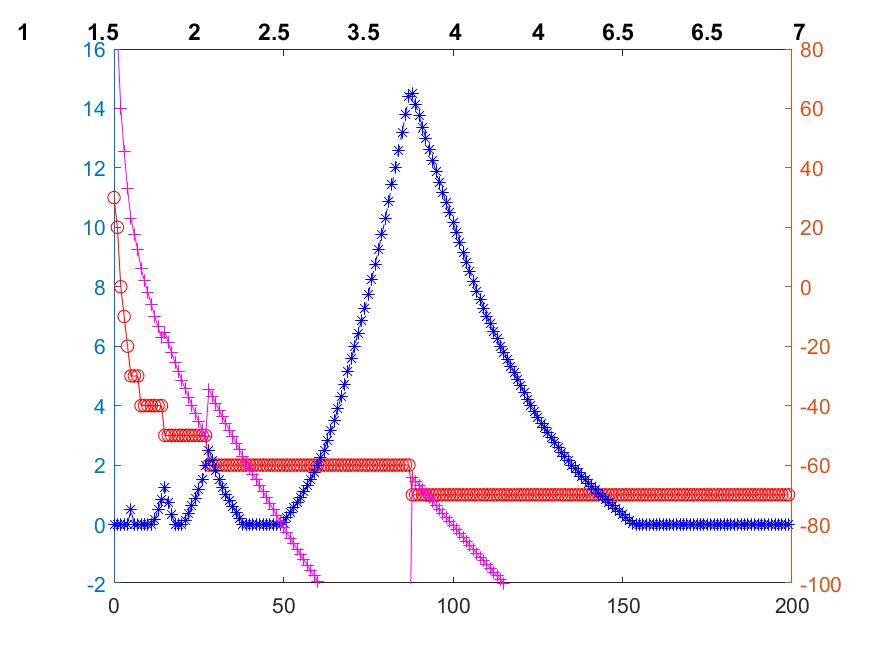
\includegraphics[width=0.8\linewidth]{Figures/Image30}  %插入的图,包括JPG,PNG,PDF,EPS等,放在源文件目录下
	\caption{机器数量和补贴随启动成本变化图}  %图片的名称
	\label{fig:Image1}   %标签,用作引用
\end{figure}

所有参与者的处理时间从小到大排列在图形的上方。红色和蓝色的线则分别代表着机器数量和补贴值。横坐标代表启动成本。左侧的纵坐标则代表机器数量的值,而右侧的纵坐标则表示补贴值。


\begin{thm}\label{thm4}

对于机器调度博弈,当使用的机器数量为1时,断点数量为 $O(v^2)$。
% 对于 机器数量为 2,3 时,证明相应的方案变化种类要少。
\end{thm}

\begin{pf}[引理2]

对于$\left| s \right|= n-1 $时的n个等式并且结合 $\alpha(V)=c(V)+P_1$ 可以得到 $\alpha(i)$ 的取值。
则对任意$\left| s' \right| < n-1$,假设$s'=\{i,\cdots,j\}$,则需证
\begin{equation} \label{lem2_1}
  \alpha(i,\cdots,j) \leq c(i,\cdots,j)+P_1
\end{equation}

代入$P_1$的值,$P_1=\alpha(V)-c(V)$,记$c(-i)=c(\{1,\cdots,i-1,i+1,\cdots,n\})$,并且代入$\alpha(i) = c(V)-c(-i)$ 于(\ref{lem2_1})式中,则只需证明下式:
\begin{equation}   \label{lem2_2}
  \sum_i^{N\setminus s'} c(-i) \leq (n-1-\left| s' \right|)c(V)+c(s')
\end{equation}

\Rightarrow \qquad

\begin{equation*}
  c(-k)-c(s') \leq (n-1-\left| s' \right|)c(V)-\sum_i^{N\setminus s'\setminus k} c(-i)
\end{equation*}

则由超模性,我们有下列一组不等式
\[
\begin{cases}
  c(V)-c(-t) \geq & c(-k)-c(-k-t) \\
  c(V)-c(-m) \geq & c(-k-t)-c(-k-t-m) \\
 \quad   \vdots        &\vdots\\
 c(V)-c(-s) \geq & c(s' \cup s)-c(s')
\end{cases}
\]
将这$(n-1-\left| s' \right|)$个不等式相加后,我们得到
$(n-1-\left| s' \right|)c(V)- \sum_i^{N\setminus s'} c(-i)+c(s') \geq 0 $。
故引理\ref{lem2}成立,即对$\forall s'$当$\left|s' \right|<n-1$时,$\alpha(s') \leq c(s')+P_1$均成立。\qed

\end{pf}


\begin{pf}[引理3]

当特征函数c(s)是超模的时,根据引理2的证明,同样我们令$c(-i)$表示大联盟中除去第i个参与者的不包含启动成本的总成本,即有$c(-i)=c(\{1,\cdots,i-1,i+1,\cdots,n\})$。\\
根据$\left| s \right|= n-1 $时的n个等式,将这n个等式相加易得$(n-1)\alpha(V)=nP_1+ \sum_{m=1}^n c(-m)$。
同时当$c(V)=\alpha(V)$时,令$\Delta m=c(V)-P_1-c(-m)$,即$\Delta m$表示参与者m对于大联盟的边际成本。\\
则有$nc(V)=nP_1+\sum_{m=1}^n c(-m) +\sum_{m=1}^n \Delta m$ \\
\Rightarrow  \qquad  $(n-1)\alpha(V)=nc(V)-\sum_{m=1}^n \Delta m$ \\
\Rightarrow   \qquad  $c(V)= \sum_{m=1}^n \Delta m$。 \\
而$c(V)=P_1+\sum C_m$,$\sum C_m $则表示从空集开始每次增加一个参与者直至形成大联盟时所有这样n个边际成本的加和。当特征函数c(s)满足超模性时,这时自然有$\sum_{m=1}^n \Delta m > \sum C_m$,这样我们就能得到此时 $P_1 > 0$。
\qed
\end{pf}


\begin{pf}[定理1]

为了表述的方便,我们设当机器数量改变时区间端点处的启动成本为 $S_{1},S_{2}, \dots ,S_{n}$。并且 $S_{i}$ 分别表示当机器数量从 $i$ 改变到 $i-1$ 时启动成本的大小。特别地,$S_{1}$ 表示当机器数量为1并且对应的补贴为0时的最小启动成本。于是我们有下面的等式:
\begin{displaymath}
  S_{1}=S_{2}+\cdots+S_{n}=\sum_{i=2}^n S_i.
\end{displaymath}
注意到,
\begin{displaymath}
  (n-1) \sum_{s \in S \setminus\{V\} } \rho_s \geq
  \sum_{k\in V}\sum_{s \in S \setminus\{V\}:k \in s} \rho_s = n
\end{displaymath}

左边的不等式意味着对于每一个 $\rho_s$ 可以最多出现$(n-1)$次,所以我们可以得到当且仅当对于每一个$\rho_s > 0$ 出现 $n-1$ 次时,等式成立。这就是说,所有包含 $n-1$ 个参与者的联盟均为最大的不满意联盟。这样,由互补松弛性我们就可以得到 $n \choose n-1$ 个等式。
\[
\begin{cases}
 \alpha_1+\alpha_2+ \cdots+\alpha_{n-1} & = x_1 \\
 \alpha_1+\alpha_3+ \cdots+\alpha_n & = x_2 \\
 \quad   \vdots        &\vdots\\
 \alpha_2+\alpha_3+ \cdots+\alpha_n & = x_n.
\end{cases}
\]
将这 $n$ 个等式加在一起,我们可以得到
\begin{equation*}
  (n-1)(\alpha_1+\alpha_2+ \cdots+\alpha_n)=\sum_{i=1}^{n}x_i
\end{equation*}
而我们已经知道,$x_1,x_2,\dots,x_n$ 可以被表示为如下的形式:
\[
\begin{cases}
x_1 = S_0 + (n-1)t_1 + (n-2)t_2 + &\cdots + t_{n-1} \\
x_2 = S_0 + (n-1)t_1 + (n-2)t_3 + &\cdots + t_{n-1} \\
\quad   \vdots        &\vdots\\
x_n = S_0 + (n-1)t_2 + (n-2)t_3 + &\cdots + t_{n}
\end{cases}
\]

根据SPT规则,我们可以得到等式 $c(V)=\alpha_1+\alpha_2+\cdots+\alpha_n=S_0+nt_1+(n-1)t_2+\dots+t_n$。
再用 $x_1,x_2,\dots,x_n$ 来代换 $c(V)$,我们可以得到只包含有 $S_0,x_1,x_2,\dots,x_n$ 的一个等式。
最终,我们得到 $S_0 = \sum_{k=1}^n (n-k)t_k$ 。
\qed
\end{pf}

\section{一种更为特殊的例子}
对于每一种 $m_V$ 对应着一种排列方式,因而我们可以借此求出每一个 $S_i$,即通过比较设施数量彼此相邻的成本。而对应到每一个子联盟,由于从 $n$ 个人中取出 $k$ 个有 $C^k_n$种取法,因而会造成指数上求解的困难,但从最简单的角度入手,如果n个人地位相同,我们希望从中得到一些有趣的性质。由于每个人平权,则我们可以将处理时间化简为都是1,即$t_i=1, \text{对所有} i \in V$, 这并不影响最终的结果。
\par
以n=9为例,当$ S_0 \in [7,20]$ 时,$m_V=2$。
$6 \leq S_0 < 9 $时,$1 \sim 5$个人的联盟均使用一台设施。
$9 \leq S_0 < 12 $时,$1 \sim 6$个人的联盟均使用一台设施。
$12 \leq S_0 < 16 $时,$1 \sim 7$个人的联盟均使用一台设施。
$16 \leq S_0 < 20 $时,$1 \sim 8$个人的联盟均使用一台设施。
可以证明当n为任意数时,都有对应的有效约束中子联盟只使用一台机器。
此时我们可以完美刻画我们需要的图形,即在什么时候存在断点以及斜率的变化情况,这些均与更一般的情况相呼应。


\begin{pf}[定理2]

由(\ref{dual})式,我们知道在启动成本为 $S_i$ 时的斜率值为$m_v-\sum_{s\in S \setminus\{V\}} \rho_s \cdot m_s$。而在 $S_i$ 左侧 机器数量$m_v=i$ 斜率为正,绝对值为$i-\sum_{s\in S \setminus\{V\}} \rho_s \cdot m_s$,右侧 机器数量$m_v=i-1$,斜率为负,绝对值为
$\sum_{s\in S \setminus\{V\}} \rho_s \cdot m_s - (i-1) $。所以 $S_i$ 左右两侧斜率绝对值之和为1。\\
当机器数量为1时,此时斜率为 $1-\sum_{s\in S \setminus\{V\}} \rho_s \cdot m_s$,由于$m_s \leq m_v$,故$m_s=1$,斜率值为 $1-\sum_{s\in S \setminus\{V\}} \rho_s $。又在$S_2$处左右两侧斜率绝对值之和为1,故右侧斜率绝对值小于1。同时又由定理1,我们有

\begin{displaymath}
  (n-1) \sum_{s \in S \setminus\{V\} } \rho_s \geq
  \sum_{k\in V}\sum_{s \in S \setminus\{V\}:k \in s} \rho_s = n
\end{displaymath}

$\sum_{s \in S \setminus\{V\}} \rho_s $最小值为$\frac{n}{n-1}$,相对应的斜率最大值为$ 1-\sum_{s\in S \setminus\{V\}} \rho_s =-\frac{1}{n-1}$
\qed
\end{pf}



\begin{pf}[定理3]

% 关于n/2的证明,还不知道怎么表述清楚

问题:对于机器调度问题,存在排序问题而由于机器是相同的,因而与机器无关。而对于例如设施选址问题,则由于不同设施对于不同player处理时间不同,因而证明遇到问题。

同时如果对于使用(而不是给定,注意区别) m 台机器,每台机器上players 数量不超过二时,(由于机器调度特征函数满足超模性,即排序后添加一个player的边际成本越来越大,因而肯定不会超过二),而对于设施选址因为没有类似的限制,因而有可能一台设施有很多player,因为不存在边际成本越来越大。

\end{pf}


\begin{pf}[定理4]

已证,还没写。
% 有关General情形的一些性质
\end{pf}


下述猜想有待验证   \\
猜想均由 4 中的特殊例子衍生
\section*{猜想1}
此猜想是关于如何预测机器调度斜率取值范围的,即
$\sum_{\rho_s} \in (m_v-1/2,m_v+1/2)$,这样可以解释为什么当机器数量为 2 到 $\frac{n}{2}$ 时,斜率会有正有负。\\

可以构造一个算法

下述问题有待解决
\section{存在的问题}
如何说明特征函数也随着机器数量而变化   不止是集合的函数(很重要)   \\


引理4的证明。


\begin{thm}\label{thm5}

有效的不等式一定是使用一台机器。

\end{thm}

\begin{pf}[定理5]

已知当 $P$ 处于 $(P_2,P_1)$ 之间时(由于此时大联盟使用一台机器),此时所有小联盟$ s$均使用一台机器。假设定理不成立,
则当$P$逐渐减少,如从$ P_2 \to P_3$ 时,某一时刻必然先出现子联盟 $s'$ (其中$|s'| \geq 2 $)使用 2 台机器是最优的情形。此时有
$ \alpha(s') = c(s') +2P $  可以找到 $ s_1 \cup s_2 = s',s_1 \cap s_2 = \emptyset $

由于 $\alpha(s_1) \leq c(s_1) + P , \alpha(s_2) \leq c(s_2) + P $
可以推出 $ c(s_1) + c(s_2) \geq c(s') $  这与特征函数满足的超模性质相违背。

因而有效约束 均是使用一台机器。

\end{pf}

此时我们可以 设计算法 简化计算限制条件。



\end{document}
